\documentclass{article}

\usepackage[margin=1in,includefoot]{geometry}
\usepackage{fancyhdr}
\usepackage{amsmath,amssymb ,amsthm}
\usepackage[ utf8 ]{ inputenc}
\usepackage{algorithm}
\usepackage[noend]{algpseudocode}
\usepackage{graphicx}
\graphicspath{ {\string~/Desktop/} }
\algnewcommand\algorithmicforeach{\textbf{for each}}
\algdef{S}[FOR]{ForEach}[1]{\algorithmicforeach\ #1\ \algorithmicdo}

\pagestyle{fancy}
\begin{document}
\begin{titlepage}
	\begin{center}
	\line(1,0){200} \\
	[0.25 in]
	\huge{\bfseries Tema 3} \\
	[2mm]
	\line(1,0){125}\\
	[1.5cm]
	\textsc{\LARGE Mocanu Ada-Astrid\\ \& \\Ciripescu Teodor}\\
	[5mm]
	Grupa A7\\
	[10mm]
	\LARGE 10 Ianuarie 2020\\
	\end{center}
\end{titlepage}



\newpage
\section*{Problema 2}
\Large
a) \\
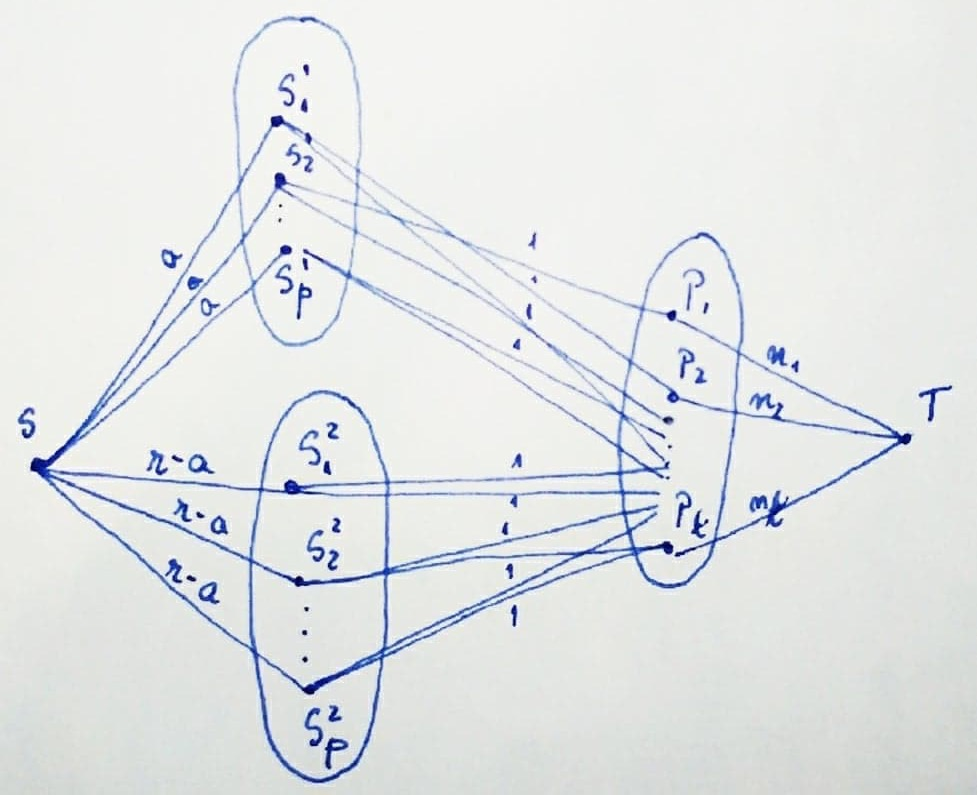
\includegraphics[width=100mm,scale=1]{2.jpg}\\
$V(G)=\{ S_1^1,S_2^1,...,S_p^1, S_1^2, S_2^2, ...,S_p^2\}\bigcap \{ P_1,P_2,...,P_k\} \bigcap \{ S,T\}$\\
$E(G)=\{S_i^1 P_j,$ daca profesorul $P_j$ este specializat in licenta studentului $S_i\} \bigcap$$\{S_i^2 P_j,$ daca profesorul $P_j$ nu este specializat in licenta studentului $S_i\} \bigcap$$\{SS_i^1, i=\overline{1,p}\}\bigcap$$\{SS_i^2, i=\overline{1,p}\}\bigcap$$\{P_jT, j=\overline{1,k}\}$\\
\bigskip\\
Fie reteaua $R=(G,S,T,c)$ a.i. $c(SS_i^1)=a,\forall i=\overline{1,p}$ , $c(SS_i^2)=r-a,\forall i=\overline{1,p}$ $c(P_jT)=n_j,\forall j=\overline{1,k}$ \\
$(S_i^1P_j)=1$, $c(S_i^2P_j)=1$\\
\bigskip\\
b) \\
Exista o asignare a profesorilor catre studentii ce dau licenta cu proprietatile cerute $\Leftrightarrow$ in $R=(G,S,T,c)$ valoarea maxima a unui flux este: $p*r$\\
$(\Rightarrow)$\\
$x(S_i^1P_j)=\begin{cases} 1, &\text{daca \($ $P_j$ este specializat in licenta lui $S_i$$\)} \\ 0, &\text{altfel} \end{cases}$\\
$x(S_i^2P_j)=\begin{cases} 1, &\text{daca \($ $P_j$ este specializat in licenta lui $S_i$$\)} \\ 0, &\text{altfel} \end{cases}$\\
$x(SS_i^1)=a,\forall i$\\
$x(SS_i^2)=r-a,\forall i$\\
$x(P_jT) \leq n_j$, unde $n_j$ este nr maxim de echipe din care poate face parte profesorul $P_j$.\\
In fiecare nod $S_i^1$ intra flux de valoare $a$(de la $S$) si iese flux de valoare $a$ din ipoteza ($\exists$ $a$ profesori specializati)\\
In fiecare nod $S_i^2$ intra flux de valoare $r-a$ si iese flux de valoare $r-a$ din ipoteza ($\exists$ $r-a$ profesori nespecializati)\\
In fiecare nod $P_j$ intra flux de valoare $q_j$ si iese flux de valoare $q_j \leq n_j$ \\
$\Rightarrow$ Fluxul creat respecta conditia de conservare si e maximal deoarece din nodul S nu poate pleca mai mult.\\
$(\Leftarrow)$\\
Fie un flux de valoare maxima $p\cdot r$, asociat retelei modelate anterior. El rezolva problema data deoarece putem considera ca nodurile $P_j$ sunt asociate profesorilor, nodurile $S_i^1,S_i^2$ sunt asociate unui student $S_i$, muchiile de la multimea $S_1$ la $P$ corespund modalitatii de alegere a celor $a$ profesori specializati, iar cele de la $S^2$ la $P$ corespund modalitatii de alegere a celor $r-a$ profesori nespecializati.\\
\bigskip\\
c)\\
$n=2+2p+k$\\
$m=2p+k+(x_1+x_2+...+x_p)+(k-x_1+k-x_2+...+k-x_p)=2p+k+(x_1+...+x_p)+kp-(x_1+...+x_p)=2p+k+kp$\\
\bigskip\\
1. Analizam algoritmul Ford $\&$ Fulkerson\\
Complexitate in general:$O(n\cdot m\cdot U)$\\
Consideram ca majorant\\
$U=r$ (pp $r>n_i,\forall i=\overline{1,k})$\\
$n\cdot m\cdot U = (2+2p+k)(2p+k+kp)r=(4p+2k+2kp+4p^2+4pk+k^2+2p^2k+k^2p)r=(4p+2k+6pk+4p^2+k^2+2p^2k+k^2p)r$\\
$\Rightarrow$ Complexitatea devine:$O(p^2kr)$, pentru $p\geq k$ sau $O(k^2pr)$, pentru $k>p$\\
\bigskip\\
\bigskip\\
2. Analizam algoritmul Edmonds-Karp\\
Complexitate generala: $O(m^2n)$\\
$m^2n=(2p+k+kp)^2(2+2p+k)=(4p^2+k^2+k^2p^2+4pk+4kp^2+2k^2p)(2+2p+k)$\\
$\Rightarrow$ Complexitatea devine: $O(k^3p^2), k\geq p$ sau $O(k^2p^3),k<p$\\
$\Rightarrow$ cum $r<k$ $\Rightarrow$ mult mai ineficient decat F\&F \\
\bigskip\\
3. Analizam algoritmul Ahuja-Orlin\\
Complexitate generala: $O(nm+n^2\log U)$\\
$nm+n^2\log U=(2p+k+kp)(2+2p+k)+(2+2p+k)^2\log r = 4p+4p^2+2pk+2k+2pk+k^2+2kp+2kp^2+k^2p+(4+4p^2+k^2+4p+2k+2pk)\log r$\\
pentru $p\geq k$$\Rightarrow$ complexitatea devine: $O(2p^2k+4p^2\log r)$\\
pentru $k>p$$\Rightarrow$ complexitatea devine: $O(k^2p+k^2\log r)$\\
In concluzie, preferam algoritmul F$\&$F.\\
\newpage
\section*{Problema 3}
\Large
3.\\
a) \\
Consideram circuitul corespunzator lui $X_{i}$\\
Orice nod alegem sa introducem intr-o prima multime, el acopera 2 muchii $\Rightarrow$\\
Nu este necesar sa introducem in aceeasi multime niciunul dintre vecinii sai directi (Cate una dintre muchiile pe care acestia le-ar putea acoperi, au fost acoperite deja de nodul curent introdus)$\Rightarrow$ Vom lua noduri din 2 in 2 si le punem in prima multime (spre exemplu, prima multime contine nodurile \{$a_{i,1}, a_{i,2}, ..., a_{i,k_i}$\})\\
$\Rightarrow$ cea de-a 2-a multime le va contine pe restul, adica pe \{$f_{i,1}, f_{i,2}, ..., f_{i,k_i}$\} (se procedeaza ca mai sus, alegand insa ca prim nod, un nod $f_i$)\\
Ambele multimi au cardinal $k_i$ si au proprietatea ca sunt minime.\\
\bigskip\\
b1)\\
$U$ acopera muchiile lui $G$$\Rightarrow$ $U$ acopera muchiile lui $H_j, j =\overline{1,m}$\\
Pentru a avea acces la muchiile lui $H_j$, trebuie introdus cel putin un nod din $H_j$. Insa daca introducem doar un nod, nu putem acoperi decat 2 muchii din cele 3 de acoperit.\\
Astfel, daca introducem 2 noduri este deja suficient pentru a putea acoperi cele 3 muchii de acoperit (nefiind necesar sa le introducem pe toate 3 neaparat)\\
$\Rightarrow$In multimea $U$ vom avea minim 2 noduri din $W_j$ (multimea nodurilor lui $H_j$)\\
$\Rightarrow$ $\mid U \cap V_j \mid \geq2, \forall j=\overline{1,m}$\\
\bigskip\\
b2)\\
$\mid U \cap(\bigcup\limits_{i=1}^n V_i) \mid = \mid U \cap V_1\mid + \mid U \cap V_2 \mid + ... + \mid U \cap V_n \mid$\\
cum $\mid U \cap V_1 \mid \geq k_1 $ (de la punctul a), $\mid U \cap V_2 \mid \geq k_2$, ... ,$\mid U \cap V_n \mid \geq k_n$ \\
$\Rightarrow$ $\mid U \cap(\bigcup\limits_{i=1}^n V_i) \mid \geq k_1 + k_2 + ... + k_n $\\
$k_1=$ nr aparitiilor lui $x_1$ in $C$\\
$k_2=$ nr aparitiilor lui $x_2$ in $C$\\
$...$\\
$k_n=$ nr aparitiilor lui $x_n$ in $C$\\
$\Rightarrow$ $k_1 + k_2 + ... + k_n = $ numarul aparitiilor tuturor literalilor in $C$ = numarul literalilor din fiecare clauza $*$ nr de clauze = $3*m$ \\
$\Rightarrow$ $\mid U \cap(\bigcup\limits_{i=1}^n V_i) \mid \geq 3m$\\
\bigskip\\
b3)\\
$\mid U \cap(\bigcup\limits_{i=1}^n V_i) \mid \geq 3m$ (1)\\
$\mid U \cap W_j\mid \geq 2 \Rightarrow$
$\mid U \cap(\bigcup\limits_{j=1}^m W_j) \mid \geq 2m$ (2)\\
Din (1) si (2) $\Rightarrow$  $\mid U\mid=\mid U \cap(\bigcup\limits_{i=1}^n V_i)\mid + $$\mid U \cap(\bigcup\limits_{j=1}^m W_j) \mid$$\geq5m$\\
Dar din ipoteza $\mid U\mid=5m\Rightarrow$\\
Suntem obligati ca $\mid U \cap(\bigcup\limits_{i=1}^n V_i) \mid=3m$ si $\mid U \cap(\bigcup\limits_{j=1}^m W_j) \mid=2m $\\
$\Rightarrow \mid U \cap W_j\mid=2$\\
\bigskip\\
b4)\\
Dupa completarea multimii $U$ algoritmul ne descrie o functie de adevar a.i. $\forall i, t(x_i)=true$ daca si numai daca $U\cap V_i=\{f_{i,1},f_{i,2},...,f_{i,k_i}\}$\\
Conform algoritmului, intr-o clauza $C_j$ va ramane un nod $w_{j,1}$(spre exemplu) care nu apartine lui $U$. Daca $w_{j,1}$ corespunde unui nod $x_i$ din clauza $C_j$, atunci nodul incident la muchia care-l contine pe $w_{j,1}$ este un nod $a_{i,k}$ si $a_{i,k}\in U$\\
$\Rightarrow$ $t(x_i)=true$ $\Rightarrow$ $t(C_j)=true$\\
Iar daca $w_{j,1}$ corespunde unui nod $\overline{x_i}$ din clauza $C_j$, atunci nodul incident la muchia care-l contine pe $w_{j,1}$ este un nod $f_{i,k}$ si $f_{i,k}\in U \Rightarrow t(x_i)=false$ $\Rightarrow$   $t(\overline{x_i})=true$$\Rightarrow$$t(C_j)=true$$\Rightarrow$ functia satisface toate clauzele din $C$.\\
\bigskip\\
\bigskip\\
c)\\
Din modul in care il construim pe $U$ $\Rightarrow$ din fiecare clauza adaugam 2 noduri $\Rightarrow$ in total se adauga 2*nr de clauze $=2m$ noduri.
Apoi, pentru fiecare $x_i$, daca $t(x_i)=true$, se adauga $k_i$ noduri, iar daca $t(x_i)=false$, se adauga tot $k_i$ noduri $\Rightarrow$ in total $\Rightarrow$  $\sum\limits_{i=1}^n k_i=3m$\\
$\Rightarrow$ $\mid U \mid =2m+3m=5m$\\
Ne ramane de demonstrat ca $U$ acopera tot graful $G$.\\
i) pentru fiecare clauza $\exists $ 2 noduri care apartin lui $U$ $\Rightarrow$ toate muchiile fiecarei clauze sunt acoperite.\\
ii) pentru fiecare literal $x_i$ in $U$ se gasesc fie $\{a_{i,1},a_{i,2},...,a_{i,k_i}\}$, fie  $\{f_{i,1},f_{i,2},...,f_{i,k_i}\}$ dupa cum $t(x_i)=true $ sau $false$ \\
$\Rightarrow$ cele $k_i$ noduri acopera toate muchiile unui subgraf ce defineste un literal.\\
iii) In ceea ce priveste muchiile care apartin multimilor $A$ si $F$, pentru fiecare clauza 2 muchii sunt deja acoperite, prin faptul ca $\exists$ 2 noduri din fiecare clauza care $\in U$.\\
Pentru cel de-al treilea nod dintr-o clauza, stim ca el este legat de un nod dintr-un literal.\\
Daca este legat de un nod $a_{i,p},p=\overline{1,k_i}$, atunci in clauza $C_j$ va aparea $x_i$ $\Rightarrow$
$t(x_i)=true$$\Rightarrow$$\{a_{i,1},a_{i,2},...,a_{i,k_i}\}\in U$$\Rightarrow$ $a_{i,p}\in U\Rightarrow$am acoperit muchia utilizand un nod din $U$.\\
Iar daca este legat de un nod $f_{i,p},p=\overline{1,k_i}$, atunci in clauza $C_j$ va aparea $\overline{x_i}$
$\Rightarrow$ $t(\overline{x_i})=true$$\Rightarrow$$t(x_i)=false$$\Rightarrow$$\{f_{i,1},f_{i,2},...,f_{i,k_i}\}\in U$$\Rightarrow$$f_{i,p}\in U$$\Rightarrow$ am acoperit muchia utilizand un nod din $U$.\\
Astfel, am reusit acoperirea tuturor muchiilor lui $G$ $\Rightarrow$ $U$ are proprietatea ceruta.\\

\newpage
\section*{Problema 4}
\Large
a)\\
Dandu-se graful $G$, consideram o $\chi(G)$-colorare(colorare minimala a nodurilor lui $G$).\\
Alegem o culoare $X$.\\
Niciun nod de culoare $X$ nu poate fi adiacent cu un alt nod de culoare $X$ (asta ar incalca principiul colorarii nodurilor)\\
$\Rightarrow$ Toate nodurile de culoarea $X$ fac parte dintr-o multime stabila.\\
Incercam adaugarea de noi noduri la multimea culorii $X$.\\
Nu puteam alege niciun nod adiacent cu vreun nod de culoare $X$ $\Rightarrow$ Vom cauta printre nodurile care nu au vecini in multimea culorii $X$. Cand gasim un astfel de nod, ii schimbam culoarea in $X$, pastrand proprietatea de multime stabila si minimalitatea colorarii ( nu este introdusa nicio culoare noua).\\
Se repeta procedeul pana cand nu se mai pot adauga noduri, obtinand in acest fel o multime stabila maximala pentru cel putin una din clasele de colorare.\\
\bigskip\\
b)\\
Daca $x$ si $y$ au aceeasi culoare $\Rightarrow$\\
(1) $\chi(G)=\chi(G\mid xy)$\\
(2)$\chi(G) \leq \chi(G+xy)$ (adaugam o culoare noua cu care il coloram pe unul din ei)\\
(3)$\chi(G)=\chi(G+xy)$\\
(4)$\chi(G) \leq \chi(G\mid xy)$ (adaugam o culoare noua cu care sa coloram nodul rezultat)\\
Din (1),(2) $\Rightarrow$ $\chi(G)=\chi(G\mid xy)\leq \chi(G+xy)$\\
Din (3),(4) $\Rightarrow$ $\chi(G)=\chi(G+xy)\leq \chi(G\mid xy)$\\
$\Rightarrow$ in ambele cazuri se alege minimul dintre cele 2\\
$\Rightarrow$ $\chi(G)=min\{\chi(G+xy),\chi(G\mid xy)\}$\\
\end{document}









